\documentclass{standalone}
\usepackage{pgfplots}
\pgfplotsset{compat=newest}

\begin{document}
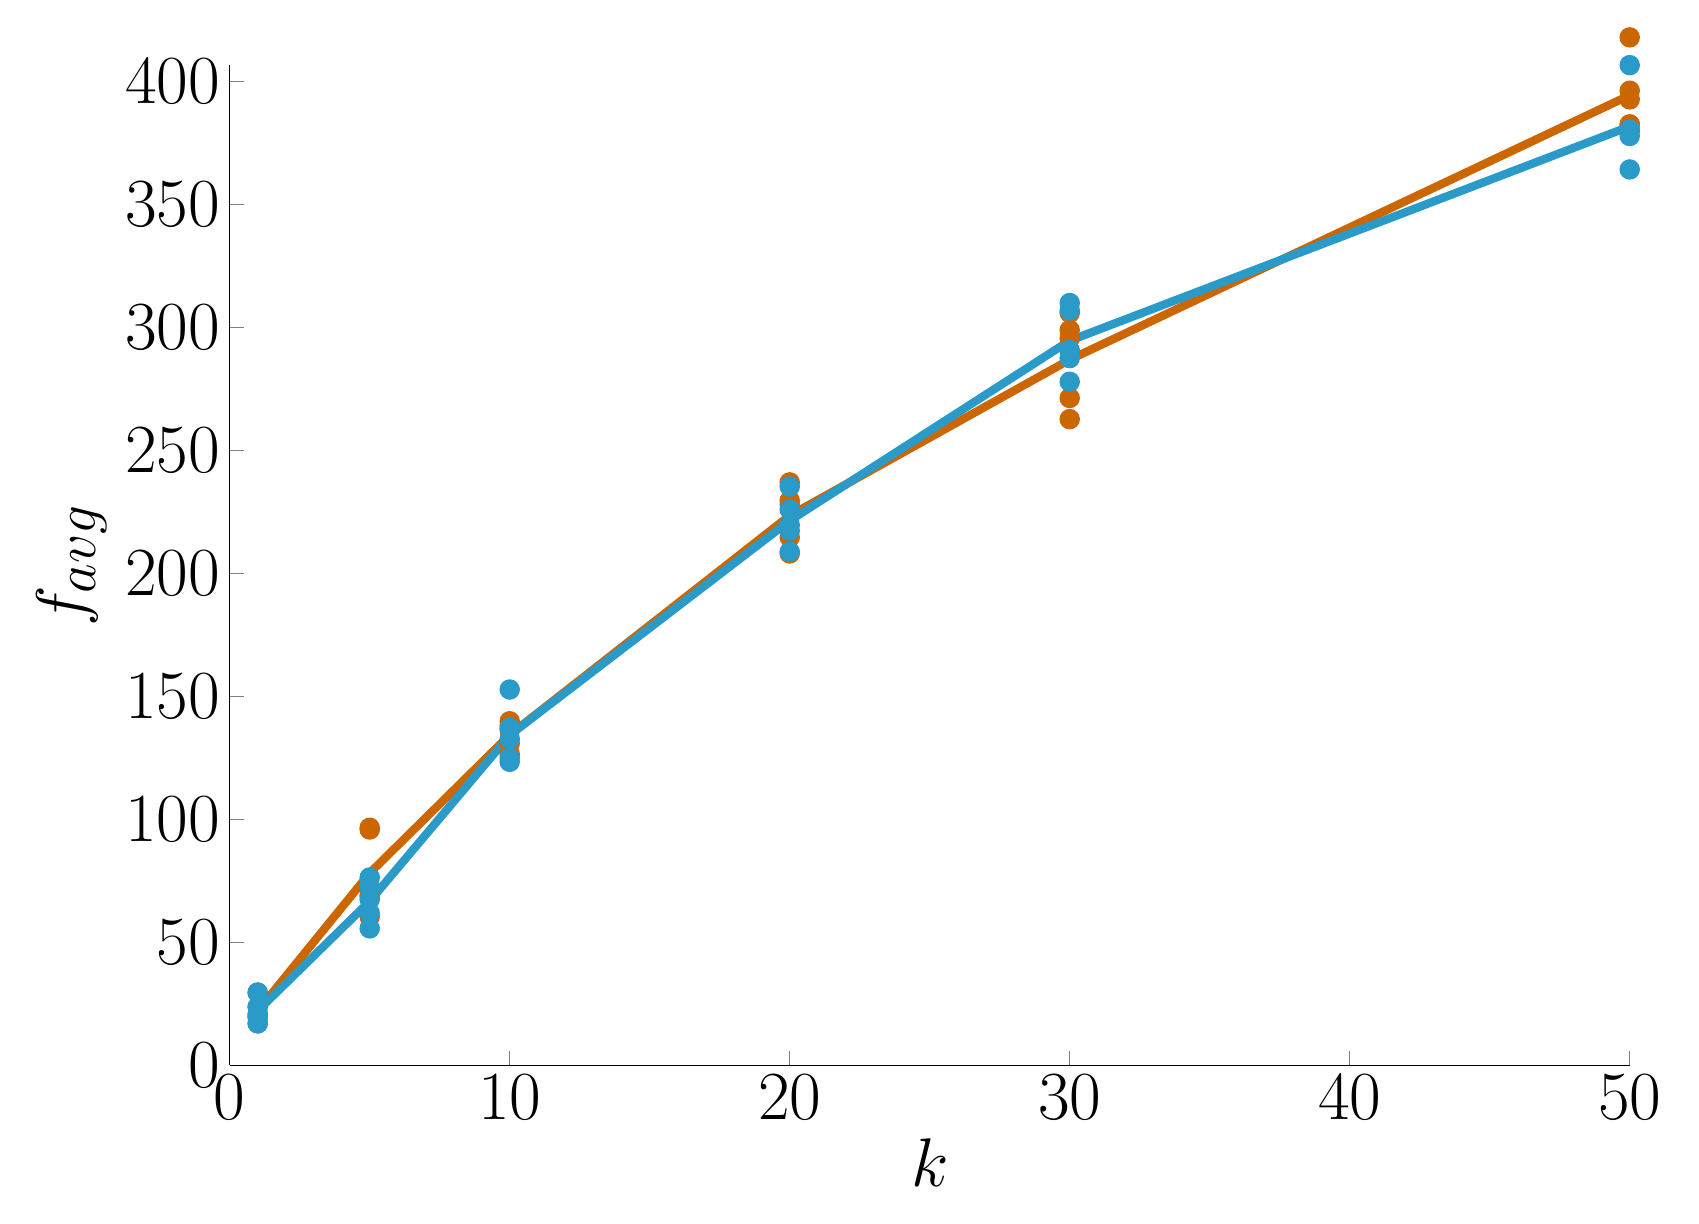
\begin{tikzpicture}

\begin{axis}[%
tick label style={font=\Huge},
label style={font=\Huge},
legend style={font=\Huge},
view={0}{90},
max space between ticks=50pt,
width=7in,
height=5in,
scale only axis,
xmin=0, xmax=50,
xtick={0, 10, 20, 30, 40, 50},
xlabel={$k$},
ymin=0, ymax=406.5,
%ytick={0, 200, 400, 600, 800, 1000},
ylabel={$f_{avg}$},
major tick length=5pt,
axis lines*=left,
legend cell align=left,
clip=false]

\addplot [
only marks,
mark=*,
mark size=3.5pt,
color=orange!80!black,
%solid,
%line width=2pt,
]
coordinates{
(1,17.0)(1,19.5)(1,20.7)(1,23.7)(1,29.5)(5,60.3)(5,68.7)(5,69.1)(5,95.8)(5,96.5)(10,126.4)(10,130.8)(10,136.3)(10,138.0)(10,139.8)(20,208.0)(20,214.6)(20,227.9)(20,229.5)(20,236.9)(30,262.6)(30,271.2)(30,295.5)(30,298.8)(30,305.8)(50,382.4)(50,382.4)(50,392.6)(50,396.1)(50,417.8)
};

\addplot [
only marks,
mark=*,
mark size=3.5pt,
color=cyan!80!black,
%solid,
%line width=2pt,
]
coordinates{
(1,17.0)(1,19.5)(1,20.7)(1,23.7)(1,29.5)(5,55.6)(5,61.8)(5,67.4)(5,72.2)(5,76.3)(10,123.3)(10,124.9)(10,132.7)(10,137.1)(10,152.7)(20,208.7)(20,217.3)(20,219.6)(20,225.9)(20,235.2)(30,277.8)(30,287.4)(30,290.7)(30,306.8)(30,309.8)(50,364.1)(50,377.7)(50,379.4)(50,380.3)(50,406.5)
};

\addplot [
color=orange!80!black,
solid,
line width=3pt
]
coordinates{
(1,22.08)(5,78.08)(10,134.26)(20,223.38)(30,286.78)(50,394.26)
};

\addplot [
color=cyan!80!black,
solid,
line width=3pt
]
coordinates{
(1,22.08)(5,66.66)(10,134.14)(20,221.34)(30,294.5)(50,381.6)
};


\end{axis}
\end{tikzpicture}
\end{document}
